\section{Introduction}
\begin{frame}[fragile]
    \frametitle{Motivating example}
    \begin{figure}[htbp]
        \centering
        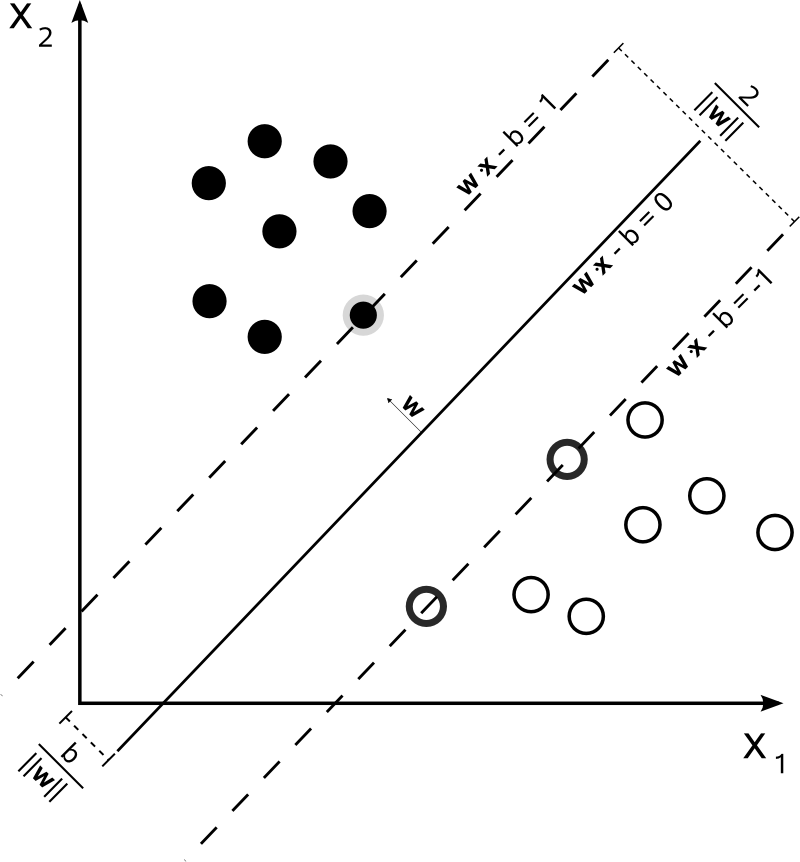
\includegraphics[height=0.8\textheight, width=0.7\textwidth]{images/svm_ex.png}
    \end{figure}
\end{frame}

\begin{frame}{Family Support Machine}
    \begin{figure}[htbp]
        \centering
        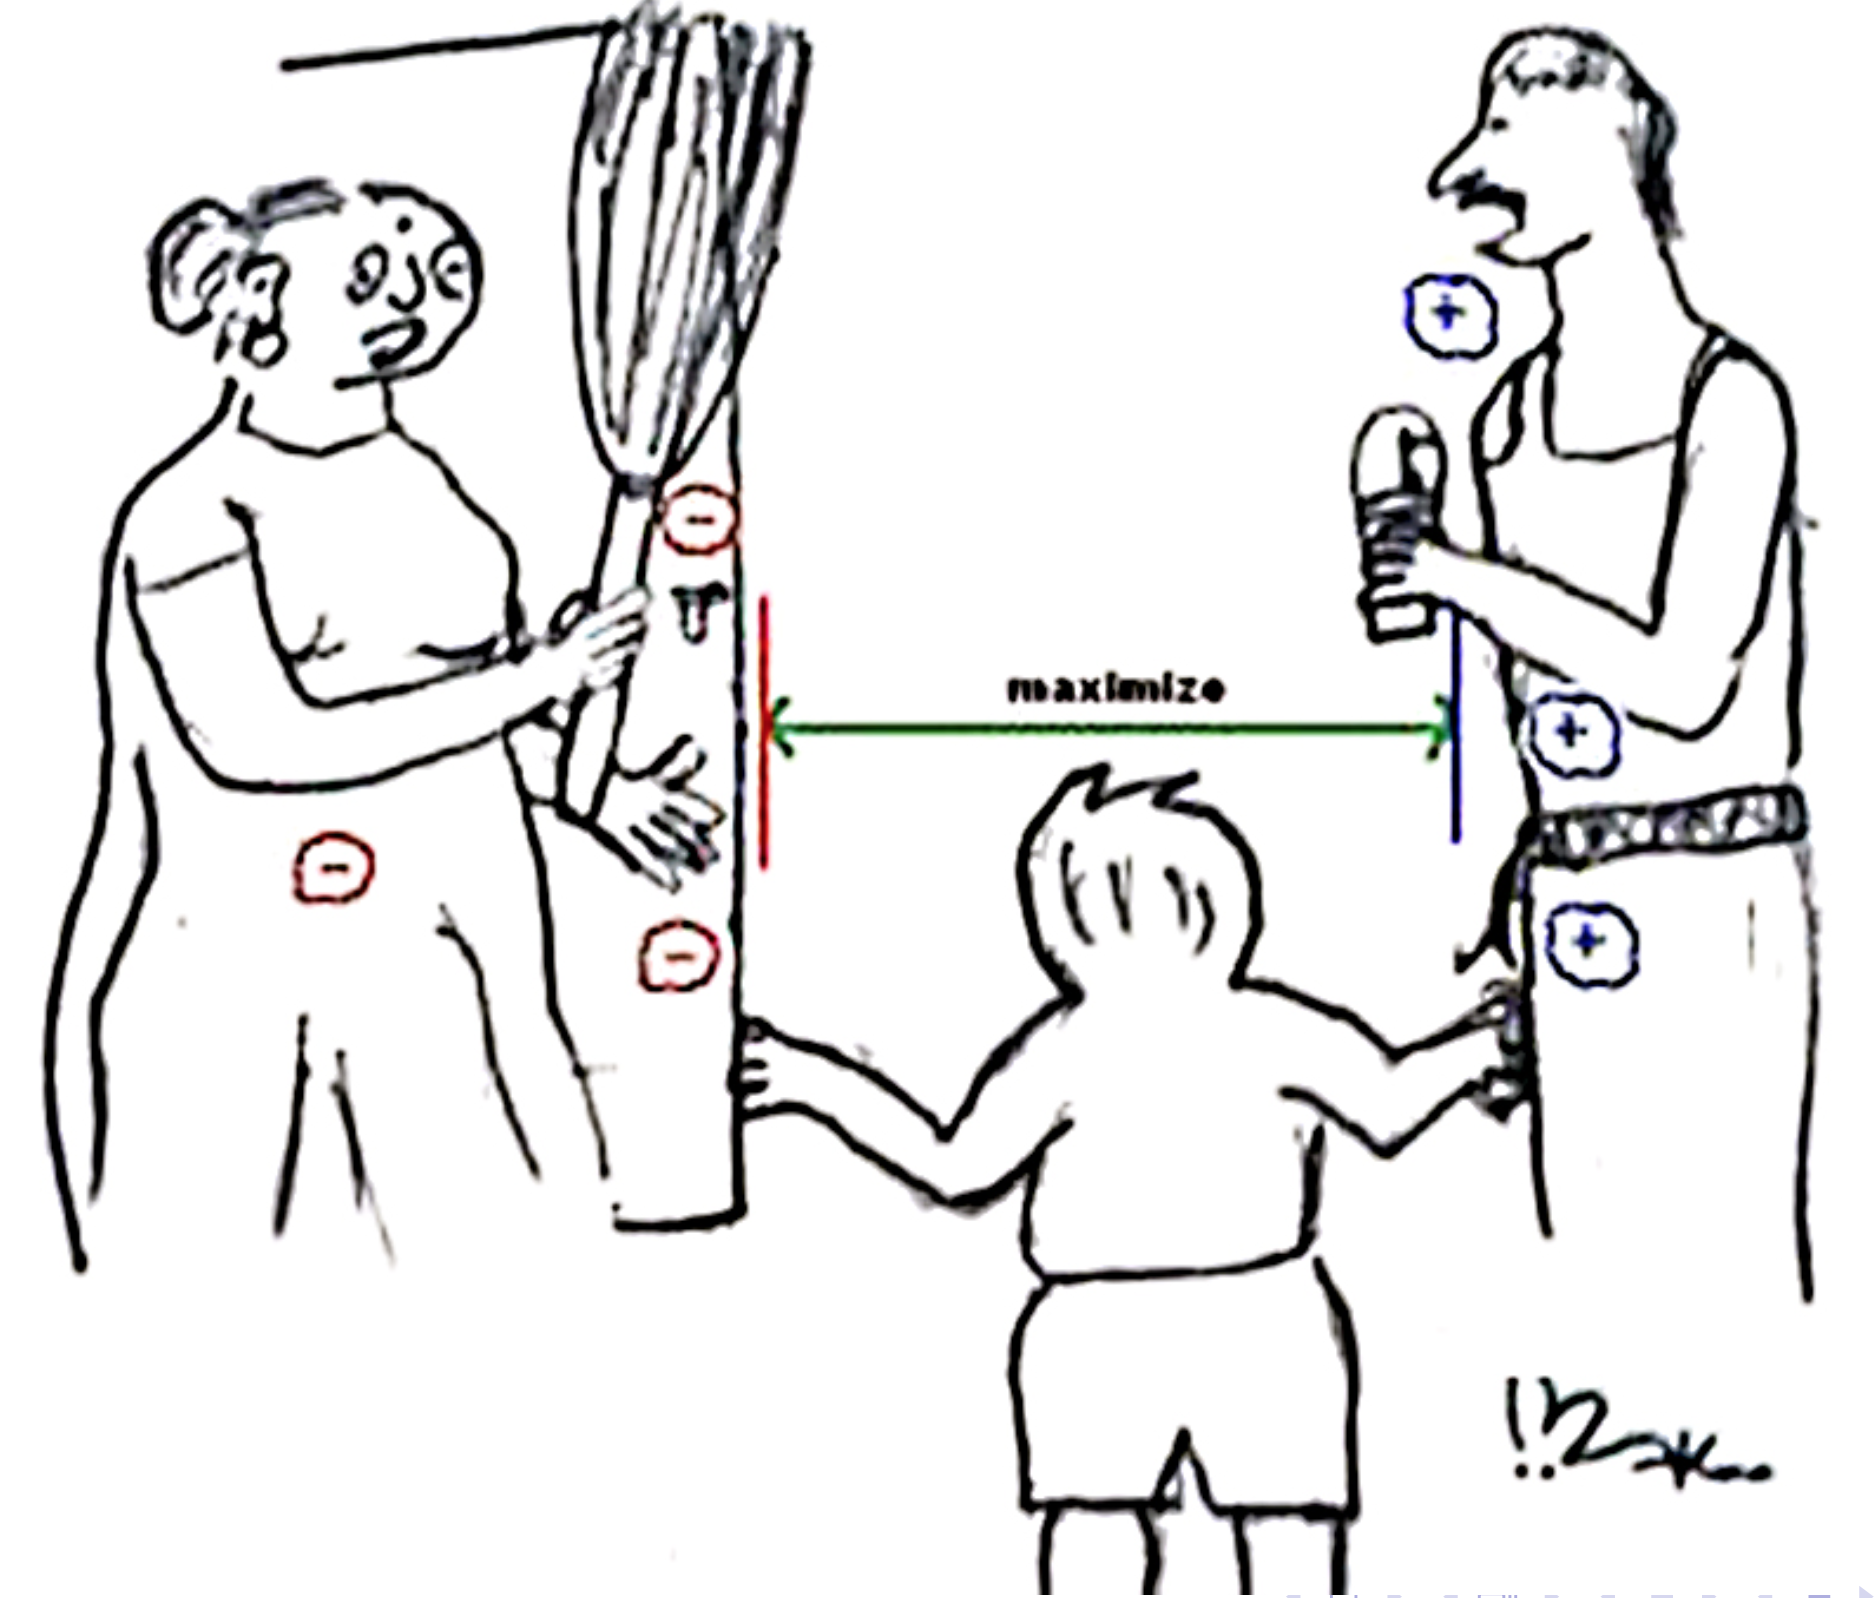
\includegraphics[height=0.6\textheight, width=0.7\textwidth]{images/family.png}
    \end{figure}
    From Peter Richt\'arik's slides
\end{frame}

\begin{frame}{Support Vector Machine: Primal Problem}
    Data: 
    \[
        \{(\xv_i,y_i)\in \R^d \times \{+1, -1\}: i\in S \overset{def}{=} \{1,2,\ldots,n\}\}
    \]
    \begin{itemize}
        \item[$\rhd$] Example: $\xv_1,\ldots,\xv_n$ (assumption: $\max_i\|\xv_i\|_2\le R$)
        \item[$\rhd$] Labels: $y_i \in\{+1,-1\}$
    \end{itemize}
    {\color{red} Optimization formulation of SVM:}
    \[
        \min_{\wv\in\R^d} \{ f(\wv):= \hat{L}_S(\wv)+\frac {\lambda} {2} \|\wv\|^2 \}
    \]
    where 
    \begin{itemize}
        \item[$\rhd$] $\hat{L}_A(\wv) \overset{def}{=} \frac{1}{|A|} \sum_{i\in A} L_i$ (average loss on examples in A)
    \end{itemize}
\end{frame}

\begin{frame}{Loss Function and Subgradient}
    \begin{block}{Definition}
        \begin{itemize}
            \item Loss: $L_i := \ell(\langle \xv_i, \wv \rangle, y_i)$

            \item Subgradient: $l'(\langle \xv_i, \wv \rangle, y_i)$ with the assumption of $\|l'\| \le \mathbb{L}$
        \end{itemize}
    \end{block}
    Use the notation $z=\langle \wv, \xv_i\rangle$, sample loss functions:
    \begin{table}[h]
        \begin{tabular}{|l|l|}
            \hline
            Loss function & Subgradient  \\ \hline
            $l(z,y_i) = \max\{0,1-y_i z\}$ & $l' = \left\{
            \begin{matrix} -y_i \xv_i & \text{if } y_i z<1 \\ 
            0 & \text{otherwise}
            \end{matrix}
        \right\}$ \\ \hline
        $l(z,y_i) = \log(1+e^{-y_iz})$ & $l' = -\frac{y_i}{1+e^{y_i z}}\xv_i$\\ \hline
        $l(z,y_i) = \max\{0, | y_i - z| - \epsilon\}$ & $l'=\left\{ 
        \begin{matrix}
            \xv_i & \text{if } z-y_i > \epsilon \\
            -\xv_i & \text{if } y_i-z > \epsilon \\
            \bm{0} & \text{otherwise}
        \end{matrix}
        \right\}$ \\ \hline
        \end{tabular}
    \end{table}
\end{frame}

